\documentclass[UTF8,12pt]{ctexart}
 
\usepackage{listings}
\usepackage{xcolor} 
\usepackage{graphicx}
\usepackage{booktabs} %绘制表格
\usepackage{caption2} %标题居中
\usepackage{geometry}
\usepackage{array}
\usepackage{amsmath}
\usepackage{subfigure} 
\usepackage{longtable}
\usepackage{abstract}
\usepackage{fancyhdr} %调用宏包
\usepackage{float}
\usepackage{hyperref}

\lstset{
basicstyle=\scriptsize,%
escapeinside=``,%
keywordstyle=\color{red} \bfseries,% \underbar,%
identifierstyle={},%
commentstyle=\color{blue},%
stringstyle=\ttfamily,%
%labelstyle=\tiny,%
extendedchars=false,%
linewidth=\textwidth,%
numbers=left,%
numberstyle=\tiny \color{blue},%
frame=trbl%
}

\geometry{a4paper,left=2.5cm,right=2.5cm,top=2.5cm,bottom=2.5cm}
\lstset{
		numbers=left, %设置行号位置
		numberstyle=\tiny, %设置行号大小
		keywordstyle=\color{blue}, %设置关键字颜色
		commentstyle=\color[cmyk]{1,0,1,0}, %设置注释颜色
		escapeinside=``, %逃逸字符(1左面的键),用于显示中文
		breaklines, %自动折行
		extendedchars=false, %解决代码跨页时,章节标题,页眉等汉字不显示的问题
		xleftmargin=1em,xrightmargin=1em, aboveskip=1em, %设置边距
		frameround=tttt,
		tabsize=4, %设置tab空格数
		showspaces=false %不显示空格
	}
 
 
\setlength{\absleftindent}{0pt}
\setlength{\absrightindent}{0pt}

\title{\vspace{-1.9cm}\textbf{武汉大学国家网络安全学院教学实验报告}}
\date{\vspace{-2.5cm}}

\pagestyle{fancy}
\fancyhead[L]{
\begin{minipage}[c]{0.04\textwidth}
  
\includegraphics[height=3.5mm]{whulogo}
\end{minipage}
\begin{minipage}[c]{0.4\textwidth}
  {\bfseries 操作系统实验报告}
\end{minipage}
}
\fancyhead[R]{2班1组}

\begin{document}
    \maketitle
    \thispagestyle{fancy}
    
    %% 头部表格
    \begin{table}[H]
    \centering
    \begin{tabular}{|p{2.5cm}<{\centering}|p{4.5cm}<{\centering}|p{3cm}<{\centering}|p{2.5cm}<{\centering}|}
    \hline
    \textbf{课程名称} & 操作系统设计与实践     & \textbf{实验日期} & 2022.10.3   \\ \hline
    \textbf{实验名称} & 分页机制          & \textbf{实验周次} & 第三周         \\ \hline
    \textbf{姓名}   & \textbf{学号}   & \textbf{专业}   & \textbf{班级} \\ \hline
    李心杨 & 2020302181022 & 信息安全   & 2    \\ \hline
    王宇骥 & 2020302181008 & 信息安全   & 2    \\ \hline
    林锟扬  & 2020302181032 & 信息安全 & 2     \\ \hline
    郑炳捷 & 2020302181024 & 信息安全 & 2     \\ \hline
    \end{tabular}
    \end{table}
    
    \section{实验目的及实验内容}
    \subsection{实验目的}
    掌握分页机制。
    
    \subsection{实验内容}
    
    \begin{enumerate}
    \item 认真阅读章节资料,掌握什么是分页机制。
    
    \item 调试代码,掌握分页机制基本方法与思路。(代码3.22中,212行---237行,设置断点调试这几个循环,分析究竟在这里做了什么?)
    
    \item 掌握PDE,PTE的计算方法。(动手画一画这个映射图;为什么代码3.22里面,PDE初始化添加了一个PageTblBase(Line 212),而PTE初始化时候没有类似的基地址呢(Line224)?)
    
    \item 熟悉如何获取当前系统内存布局的方法。
    
    \item 掌握内存地址映射关系的切换。(画出流程图)
    
    \item 基础题:依据实验的代码,(1)自定义一个函数,给定一个虚拟地址,能够返回该地址从虚拟地址到物理地址的计算过程,如果该地址不存在,则返回一个错误提示。(2)完善分页管理功能,补充alloc\_pages, free\_pages两个函数功能,试试你能一次分配的最大空间有多大,如果超出了有什么办法解决呢?
    
    \item 进阶题(选做):设计一个内存管理器。提示,均按照页为最小单位进行分配、对于空闲空间管理可采用位图法或其他方法进行管理,分配策略不限。
    \end{enumerate}
    
    \section{实验环境及实验步骤}
    \subsection{实验环境}
    $\bullet$ Ubuntu 16.04.1;
    
    $\bullet$ VMWare Workstation 16 player;
    
    $\bullet$ bochs 2.7。
    
    \subsection{实验步骤}
    \begin{enumerate}
        \item 调试代码pmtest6.asm,设置恰当的断点查看循环,总结分页机制的基本方法与思路。
        \item 运行代码pmtest7.asm,熟悉得到内存布局信息的方法。
        \item 调试pmtest8.asm,体会分页,掌握内存地址映射关系的切换。
        \item 编写函数,给定一个虚拟地址能够返回该地址从虚拟地址到物理地址的实验过程。
        \item 选用伙伴策略,设计一个内存管理器。
    \end{enumerate} 
    
    
    \section{实验过程分析}
    \subsection{调试pmtest6.asm}
    \subsubsection{阅读代码}
    先观察pmtest6.asm。代码大致分为gdt段、数据段、全局堆栈段、进入保护模式前的16位代码段、32位代码段、退出保护模式后的16位代码段。代码运行的流程图大致如图\ref{pmtest6}所示。
    \begin{figure}[ht]
        \centering
        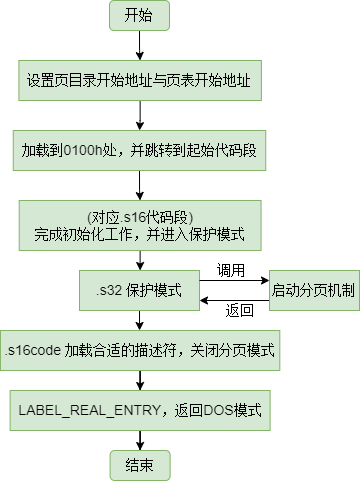
\includegraphics[width=8cm]{images/pmtest6.png}
        \caption{pmtest6流程图}
        \label{pmtest6}
    \end{figure}
    
    很多部分是与pmtest2.asm是相同的,这里不再赘述。下面阐释SetupPaging关键代码细节。
    
    阅读下文中的代码段。第6-9行是让段寄存器es对应页目录表段,再将edi设置为0,此时es:edi就指向了目录表的开始。设置eax值为PageTblBase | PG\_P | PG\_USU |  PG\_RWW。查阅资料,stosd需要寄存器edi配合使用。每执行一次stosd,就将eax中的内容复制到[edi]中。注意edi能实现自动增减(由DF标志位决定是自增还是自减,前面的代码已经执行了cld指令设置DF=0,此时edi为自增状态)。在代码的12-15行,向存放在连续的物理地址中的PDE写入eax值,每循环1次eax增加4096(这表示所有页表在内存中是连续的),共循环1024次(对应代码的第8行)。
    
    代码的17-27行是在初始化所有页表中的PTE。共1024个页表,每个页表有1024个PTE,所以共需要循环$1024^2$次。因为在前面我们令页表在内存中连续存储,所以这里直接使用edi进行自增即可,无需跳转。循环前,令es:edi指向第0个页表的第0个PTE的地址,eax赋值为PG\_P | PG\_USU | PG\_RWW。这说明第0个页表的第0个PTE指示的页首地址为0,所以在这段程序中,线性地址被映射到同样的物理地址中。
    
    完成PDE、PTE初始化后,修改CR3的值,并且将CR0最高位置为1。此时分页机制就被启动了。
    
    \begin{lstlisting}[language={[x86masm]Assembler}]
    ; 启动分页机制 
SetupPaging:
	; 为简化处理, 所有线性地址对应相等的物理地址.

	; 首先初始化页目录
	mov	ax, SelectorPageDir	; 此段首地址为 PageDirBase
	mov	es, ax
	mov	ecx,pmtest6 1024		; 共 1K 个表项
	xor	edi, edi
	xor	eax, eax
	mov	eax, PageTblBase | PG_P  | PG_USU | PG_RWW
.1:
	stosd
	add	eax, 4096		; 为了简化, 所有页表在内存中是连续的.
	loop	.1

	; 再初始化所有页表 (1K 个, 4M 内存空间)
	mov	ax, SelectorPageTbl	; 此段首地址为 PageTblBase
	mov	es, ax
	mov	ecx, 1024 * 1024	; 共 1M 个页表项, 也即有 1M 个页
	xor	edi, edi
	xor	eax, eax
	mov	eax, PG_P  | PG_USU | PG_RWW
.2:
	stosd
	add	eax, 4096		; 每一页指向 4K 的空间
	loop	.2

	mov	eax, PageDirBase
	mov	cr3, eax
	mov	eax, cr0
	or	eax, 80000000h
	mov	cr0, eax
	jmp	short .3
.3:
	nop

	ret
; 分页机制启动完毕
    \end{lstlisting}
    
    该程序运行时,内存结构如下图所示。
    \begin{figure}[H]
        \centering
        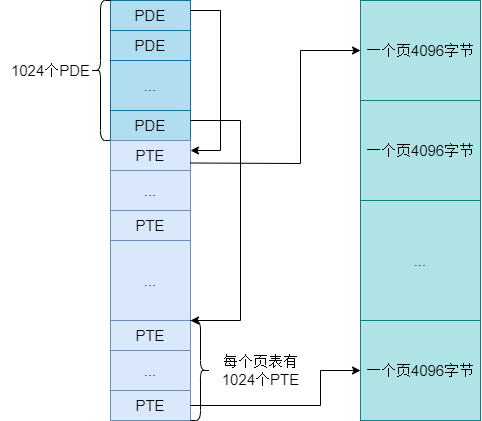
\includegraphics[width=10cm]{images/pmtest6_mem.png}
        \caption{pmtest6内存展示}
        \label{pmtest6_mem}
    \end{figure}
    
    
    \subsubsection{调试代码\label{调试PTE,PDE}}
    $\bullet$ 调试第一个循环。将.s1修改如下:
    \begin{figure}[H]
        \centering
        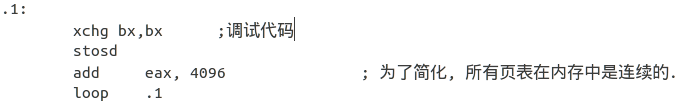
\includegraphics{images/debug1.png}
        \caption{debug第一个循环}
        \label{debug1}
    \end{figure}
    编译pmtest6.asm并装载。在bochsrc中加入magic\_break: enabled=1一行,开启调试模式。可以看到在DOS状态下运行pmtest6.com,程序停在了调试点,等待调试。
    \begin{figure}[H]
        \centering
        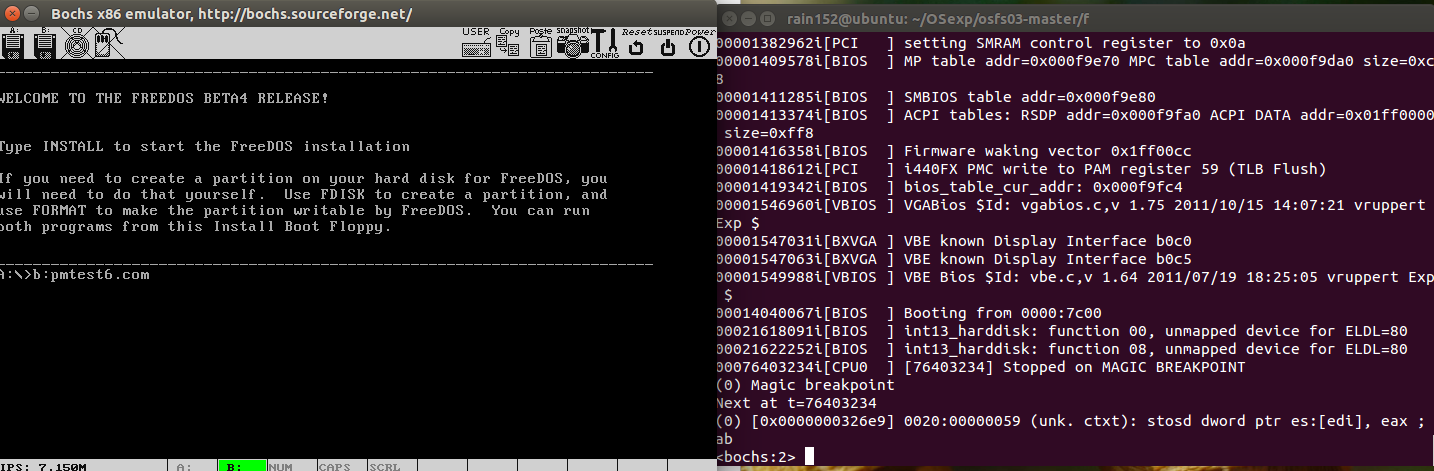
\includegraphics[width=10cm]{images/debug-status.png}
        \caption{调试模式}
        \label{debug_status}
    \end{figure}
    
    执行4层循环,查看0x00200000地址处的值。
    
    \begin{figure}[H]
        \centering
        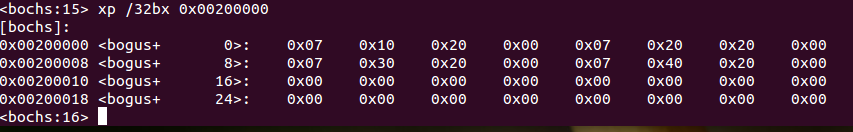
\includegraphics[width=12cm]{images/pmtest6_loop1.png}
        \label{pmtest6_loop1}
    \end{figure}
    可以看到4个PDE的内容分别是0x00201007, 0x00202007, 0x00203007, 0x00204007。这和我们在阅读代码中的理解是一致的。经过这1024层循环,所有的PDE都能够被赋为合适的值。此处不再继续调试。
    
    $\bullet$ 调试第二个循环。将.s2修改如下:
    \begin{figure}[H]
        \centering
        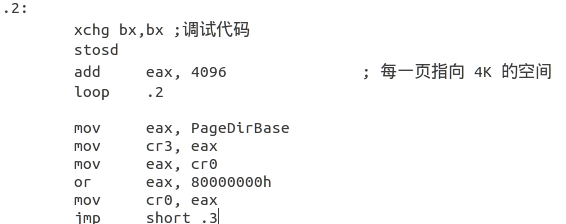
\includegraphics[width=12cm]{images/debug2.png}
        \caption{debug第二个循环}
        \label{debug2}
    \end{figure}
    
    继续在DOS中进行调试。停在调试点后,我们先查看PDE的赋值情况。可以看到PDE完成了赋值。
    \begin{figure}[H]
        \centering
        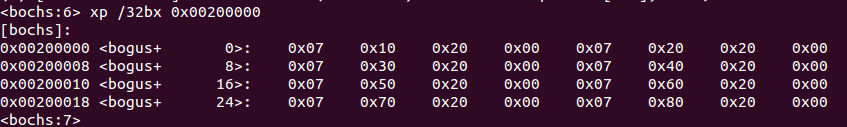
\includegraphics[width=12cm]{images/finish_PDE.png}
        \caption{PDE完成赋值}
        \label{finish_PDE}
    \end{figure}
    
    执行4层循环后,查看0x201000地址处的值(阅读代码时我们知道PTE从0x201000处开始存放)。
    
    \begin{figure}[H]
        \centering
        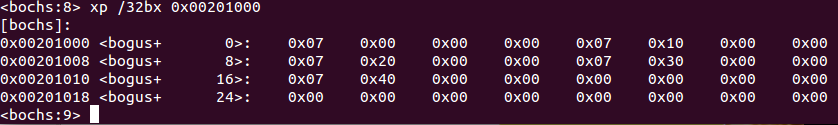
\includegraphics[width=12cm]{images/debug2_ans.png}
        \label{debug2_ans}
    \end{figure}
    可以看到前4个PTE的值分别为0x00000007, 0x00001007, 0x00002007, 0x00002007。对应的页基址0,1,2,3。PTE赋值也与我们的理解相符。经过1024*1024层循环后,所有的PTE完成赋值,进而实现将线性地址映射到对应的物理地址。
    
    $\bullet$ 运行程序。取消断点,直接运行pmtest6.com。运行结果如图\ref{result6}所说。打印的结果与pmtest2是相同的。说明程序正确运行。
    \begin{figure}[H]
        \centering
        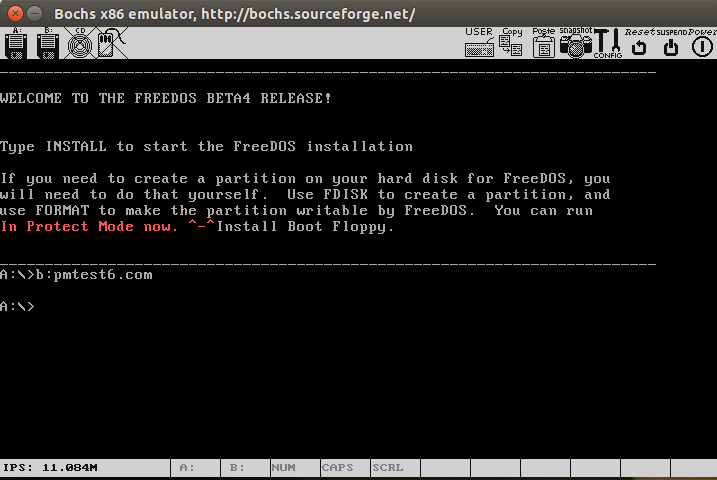
\includegraphics[width=8cm]{images/pmtest6_result.png}
        \caption{pmtest6运行结果}
        \label{result6}
    \end{figure}
    
    \subsection{运行pmtest7.asm\label{运行pmtest7}}
    \subsubsection{阅读代码}
    pmtest7.asm代码在pmtest6.asm的基础上增加了关于内存计算的一些操作。其代码流程图如图\ref{pmtest7流程图}。
    
    $\bullet$ 计算内存。相关代码如下。这段代码主要利用了int 15h来得到内存信息。更具体地说,通过该调用能够将内存信息即地址范围描述符结构ARDS写入缓冲区中,供后续输出函数使用。关于ARDS结构以及int 15h的细节这里不过多涉及。执行这段代码后,ARDS信息保存在MemChkBuf起始的缓冲区中,\_dwMCRNumber保存循环次数(也就是ARDS的总个数)。
    
    \begin{lstlisting}[language={[x86masm]Assembler}]
; 得到内存数
	mov	ebx, 0
	mov	di, _MemChkBuf
.loop:
	mov	eax, 0E820h
	mov	ecx, 20
	mov	edx, 0534D4150h
	int	15h
	jc	LABEL_MEM_CHK_FAIL
	add	di, 20
	inc	dword [_dwMCRNumber]
	cmp	ebx, 0
	jne	.loop
	jmp	LABEL_MEM_CHK_OK
LABEL_MEM_CHK_FAIL:
	mov	dword [_dwMCRNumber], 0
LABEL_MEM_CHK_OK:
    \end{lstlisting}
    
    $\bullet$ 打印内存信息。该部分代码如下。每次循环读取一个ARDS,从中抽取出对应的信息,打印在屏幕上。其中调用了DispInt和DispStr函数,它们封装在lib.inc中。循环的次数在计算内存时已经保存在dwMCRNumber指向的地址中。
    \begin{lstlisting}[language={[x86masm]Assembler}]
DispMemSize:
	push	esi
	push	edi
	push	ecx

	mov	esi, MemChkBuf
	mov	ecx, [dwMCRNumber];for(int i=0;i<[MCRNumber];i++)//每次得到一个ARDS
.loop:				  ;{
	mov	edx, 5		  ;  for(int j=0;j<5;j++) //每次得到一个ARDS中的成员
	mov	edi, ARDStruct	  ;  {//依次显示BaseAddrLow,BaseAddrHigh,LengthLow,
.1:				  ;             LengthHigh,Type
	push	dword [esi]	  ;
	call	DispInt		  ;    DispInt(MemChkBuf[j*4]); //显示一个成员
	pop	eax		  ;
	stosd			  ;    ARDStruct[j*4] = MemChkBuf[j*4];
	add	esi, 4		  ;
	dec	edx		  ;
	cmp	edx, 0		  ;
	jnz	.1		  ;  }
	call	DispReturn	  ;  printf("\n");
	cmp	dword [dwType], 1 ;  if(Type == AddressRangeMemory)
	jne	.2		  ;  {
	mov	eax, [dwBaseAddrLow];
	add	eax, [dwLengthLow];
	cmp	eax, [dwMemSize]  ;    if(BaseAddrLow + LengthLow > MemSize)
	jb	.2		  ;
	mov	[dwMemSize], eax  ;    MemSize = BaseAddrLow + LengthLow;
.2:				  ;  }
	loop	.loop		  ;}
				  ;
	call	DispReturn	  ;printf("\n");
	push	szRAMSize	  ;
	call	DispStr		  ;printf("RAM size:");
	add	esp, 4		  ;
				  ;
	push	dword [dwMemSize] ;
	call	DispInt		  ;DispInt(MemSize);
	add	esp, 4		  ;

	pop	ecx
	pop	edi
	pop	esi
	ret
    \end{lstlisting}
    
    \begin{figure}[H]
        \centering
        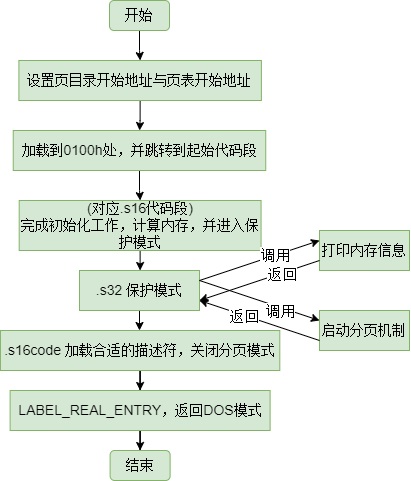
\includegraphics[width=8cm]{images/pmtest7.png}
        \caption{pmtest7流程图}
        \label{pmtest7流程图}
    \end{figure}
    
    \subsubsection{运行程序}
    对pmtest7.asm编译、装载。在DOS中运行该程序,运行结果如下图所示。
    \begin{figure}[H]
        \centering
        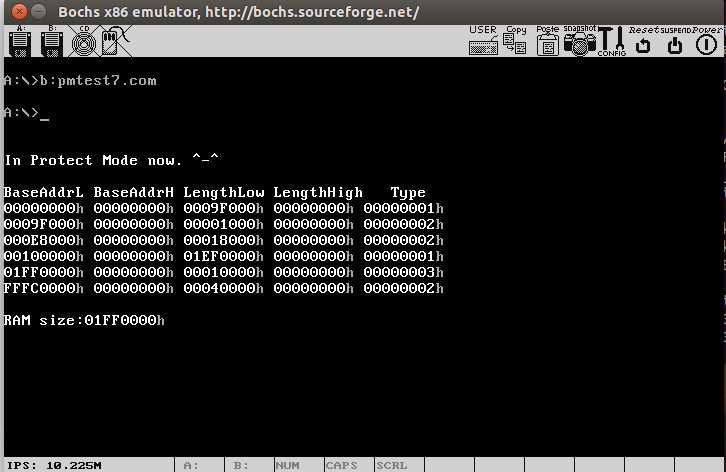
\includegraphics[width=10cm]{images/pmtest7_result.png}
        \caption{pmtest7运行结果}
        \label{pmtest7运行结果}
    \end{figure}
    
    给出这六段内存的解释。
\begin{table}[H]
\caption{内存情况}
\centering
\begin{tabular}{|c|c|c|}
\hline
{\color[HTML]{333333} \textbf{内存段}} & {\color[HTML]{333333} \textbf{属性}} & 是否可被OS使用 \\ \hline
00000000h$\sim$0009EFFFh            & AddressRangeEntry                  & 可        \\ \hline
0009F000h$\sim$000E7FFFh            & AddressRangeReserved               & 不可       \\ \hline
000E8000h$\sim$000FFFFFh            & AddressRangeReserved               & 不可        \\ \hline
00100000h$\sim$01FEFFFFh            & AddressRangeEntry                  & 可       \\ \hline
01FF0000h$\sim$FFFBFFFFh            & 未定义                                & 不可        \\ \hline
FFFC0000h$\sim$FFFFFFFFh            & AddressRangeReserved               & 不可       \\ \hline
\end{tabular}
\end{table}

    由此可得,操作系统可以使用的最大的内存地址为O1FEFFFFh,机器最大内存约为32MB。此时我们发现,32MB的内存只需要32KB的页表即可实现访问。这意味着在初始化PDE和PTE时,可以控制它们有合适的数量,这样可以有更多的空间来存储其他信息。
    
    \subsubsection{pmtest7关于PDE、PTE分配改进}
    基于前面的分析,在分配PDT空间时,可以精确计算出最合适的数量。pmtest7的SetupPaging部分的改进如下。[dwMemSize]存放机器总内存,所以执行3-5行代码后,eax中存放页表的个数(为了严谨,后面几行代码检测余数,若不为0 则需增加一个页表)。后面PTE的个数也需要进行相应修改。如此改进后,页表所占的空间小得多,程序所需的内存空间也会相应减小。
    \begin{lstlisting}[language={[x86masm]Assembler}]
SetupPaging:
	; 根据内存大小计算应初始化多少PDE以及多少页表
	xor	edx, edx
	mov	eax, [dwMemSize]
	mov	ebx, 400000h	; 400000h = 4M = 4096 * 1024, 一个页表对应的内存大小
	div	ebx
	mov	ecx, eax	; 此时 ecx 为页表的个数,也即 PDE 应该的个数
	test	edx, edx
	jz	.no_remainder
	inc	ecx		; 如果余数不为 0 就需增加一个页表
.no_remainder:
	push ecx		; 暂存页表个数
    \end{lstlisting}
    
    \subsection{运行pmtest8.asm\label{运行pmtest8}}
    \subsubsection{阅读代码}
    在前面的代码中已经实现了根据可利用内存合理分页,但是并没有利用到分页机制的优势,于是在pmtest8中通过改变地址映射关系来让在两次执行同一个线性地址的模块时产生不同的结果。其代码流程如图\ref{pmtest8流程图}。
    
    \begin{figure}[H]
        \centering
        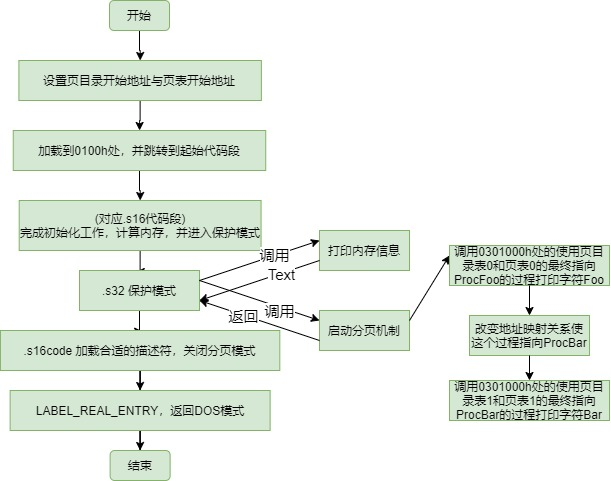
\includegraphics[width=10cm]{images/pmtest8.jpg}
        \caption{pmtest8流程图}
        \label{pmtest8流程图}
    \end{figure}
    
    除了在GDT表中使用两个不同的描述符和选择子来指向同一个Flat段来表示可执行或者读写属性以外,其相对于pmtest7的改变如下:
    
    $\bullet$ 分页机制设置:新增了一个变量页表数量PageTableNumber,方便不同的页表的初始化。修改后的SetupPaging如下:
    \begin{lstlisting}[language={[x86masm]Assembler}]
SetupPaging:
    ...
.no_remainder:
	mov	[PageTableNumber], ecx	; 暂存页表个数

	; 为简化处理, 所有线性地址对应相等的物理地址. 并且不考虑内存空洞.

	; 首先初始化页目录
	mov	ax, SelectorFlatRW
	mov	es, ax
	mov	edi, PageDirBase0	; 此段首地址为 PageDirBase0
	xor	eax, eax
	mov	eax, PageTblBase0 | PG_P  | PG_USU | PG_RWW
.1:
	stosd
	add	eax, 4096		; 为了简化, 所有页表在内存中是连续的.
	loop	.1

	; 再初始化所有页表
	mov eax, [PageTableNumber]	; 页表个数
	mov	ebx, 1024		; 每个页表 1024 个 PTE
	mul	ebx
	mov	ecx, eax		; PTE个数 = 页表个数 * 1024
	mov	edi, PageTblBase0	; 此段首地址为 PageTblBase0
	xor	eax, eax
	mov	eax, PG_P  | PG_USU | PG_RWW
.2:
	stosd
	add	eax, 4096		; 每一页指向 4K 的空间
	loop	.2

	mov	eax, PageDirBase0
	mov	cr3, eax
    ...
    \end{lstlisting}
    
    在初始化页目录和页表的过程中,ES的值始终为SelectorFlatRW,而为了简化处理,所有线性地址对应相等的物理地址,这样只需要将想取的物理地址赋值给EDI即可,在上述代码中的stosd等指令便利用了这一点。特别地,上面代码中的PageDirBase0和PageTblBase0是第0个页目录表和页表的基地址。
    
    在流程图中提到的被两次调用的过程为ProcPagingDemo,其调用指向打印字符的过程的LinearAddrDemo。相比于pmtest7,新建了函数PagingDemo来存放封装所有和分页有关的内容:
    
    \begin{lstlisting}[language={[x86masm]Assembler}]
PagingDemo:
	mov	ax, cs
	mov	ds, ax
	mov	ax, SelectorFlatRW
	mov	es, ax

	push	LenFoo
	push	OffsetFoo
	push	ProcFoo
	call	MemCpy
	add	esp, 12

	push	LenBar
	push	OffsetBar
	push	ProcBar
	call	MemCpy
	add	esp, 12

	push	LenPagingDemoAll
	push	OffsetPagingDemoProc
	push	ProcPagingDemo
	call	MemCpy
	add	esp, 12

	mov	ax, SelectorData
	mov	ds, ax			; 数据段选择子
	mov	es, ax

	call	SetupPaging		; 启动分页

	call	SelectorFlatC:ProcPagingDemo
	call	PSwitch			; 切换页目录,改变地址映射关系
	call	SelectorFlatC:ProcPagingDemo

	ret
    \end{lstlisting}
    
    其中的MemCpy类似C语言的memcpy函数,作用是将用到的三个过程到指定的内存地址中。
    
    $\bullet$ 改变地址映射关系:增加PSwitch函数来改变地址映射关系,这个函数与设置分页机制的SetupPaging类似,只是增加了改变线性地址LinearAddrDemo对应物理地址的语句。与SetupPaging中不同的是,页目录表和页表的基地址发生变化,变更为第1个:PageDirBase1和PageTblBase1(cr3的值发生了变化),从而在这个函数被调用之后能够使线性地址指向的物理地址从ProcFoo变更为ProcBar。
    
    \begin{lstlisting}[language={[x86masm]Assembler}]
PSwitch:
	; 初始化页目录
	mov	ax, SelectorFlatRW
	mov	es, ax
	mov	edi, PageDirBase1	; 此段首地址为 PageDirBase1
	xor	eax, eax
	mov	eax, PageTblBase1 | PG_P  | PG_USU | PG_RWW
	mov	ecx, [PageTableNumber]
.1:
	stosd
	add	eax, 4096		; 为了简化, 所有页表在内存中是连续的.
	loop	.1

	; 再初始化所有页表
	mov	eax, [PageTableNumber]	; 页表个数
	mov	ebx, 1024		; 每个页表 1024 个 PTE
	mul	ebx
	mov	ecx, eax		; PTE个数 = 页表个数 * 1024
	mov	edi, PageTblBase1	; 此段首地址为 PageTblBase1
	xor	eax, eax
	mov	eax, PG_P  | PG_USU | PG_RWW
.2:
	stosd
	add	eax, 4096		; 每一页指向 4K 的空间
	loop	.2

	; 在此假设内存是大于 8M 的
	mov	eax, LinearAddrDemo
	shr	eax, 22
	mov	ebx, 4096
	mul	ebx
	mov	ecx, eax
	mov	eax, LinearAddrDemo
	shr	eax, 12
	and	eax, 03FFh	; 1111111111b (10 bits)
	mov	ebx, 4
	mul	ebx
	add	eax, ecx
	add	eax, PageTblBase1
	mov	dword [es:eax], ProcBar | PG_P | PG_USU | PG_RWW

	mov	eax, PageDirBase1
	mov	cr3, eax
	jmp	short .3
.3:
	nop

	ret
    \end{lstlisting}
    
    \subsubsection{运行程序}
    如图所示,实验结果符合预期,结果中打印出了红色的Foo和Bar。分页机制使得应用程序不再直接使用物理地址,线性地址与物理地址之间的映射由操作系统负责,在一定程度上实现了内存保护。
    
    
    \begin{figure}[H]
        \centering
        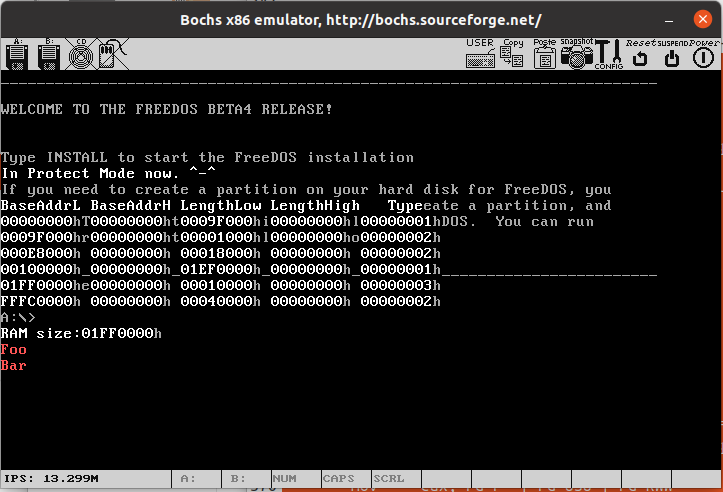
\includegraphics[width=12cm]{images/pmtest8_result.png}
        \caption{pmtest8运行结果}
        \label{pmtest8运行结果}
    \end{figure}
    
    \subsection{基础题\label{Basic page switch}} 
    \subsubsection{任务一:模拟从虚拟地址到物理地址的计算过程}
    模拟 CPU 计算物理地址的过程,逐步找到 PDE、PTE,最终用 PTE对应的物理页地址与页内偏移合并即可。
    
    实现的两个函数功能如下:
    
    \begin{enumerate}
        \item TestL2P 传入 eax 线性地址显示线性地址转化为物理地址的过程。
        \item GetL2P 返回 eax 对应的物理地址在 ebx 中,错误信息放在 ecx 中。
    \end{enumerate}
    
    其中 1 用于调试,2 用于计算。完整的代码在 libm.inc中,代码较长,不便粘贴。具体的计算过程在前面的流程描述中已经详细介绍过,此处不再赘述。此处仅描述实现中的部分细节:
    
    为了在计算过程中显示进度,TestL2P中使用了自己定义的显示函数,这些函数需要 DATA 段来支撑。本人在实现中使用了用堆栈实时保存段寄存器值的方法。以下面获取页表地址的代码为例:
    \begin{lstlisting}[language={[x86masm]Assembler}]
mov ebx, cr3
shr eax, 22
and eax, 03FFh
shl eax, 2 ; 每个页目录项占 4 个字节
push ds
mov edx, SelectorFlatRW
mov ds, edx
mov ebx, [ebx + eax]
pop ds
push ebx
call DispInt
pop ebx
ShowStr strh32
    \end{lstlisting}
    虽然在本例中,为了方便,我们将线性地址基本设置成与物理地址一一对应。而且课本在查找页表和修改页表时也没有关闭。但我们知道,我们模拟时使用的页表、页目录中存的地址,都是页的物理地址而不是虚拟地址。在分页开启的情况下模拟地址转换的过程,在逻辑上有点“自相矛盾”。因此,在程序开头,出于谨慎,我们关闭了 cr0 的分页开关。并在后面进行了恢复。
    \begin{lstlisting}[language={[x86masm]Assembler}]
...
mov eax, cr0
and eax, 7FFFFFFFh
mov cr0, eax
...
mov eax, cr0
or eax, 80000000h
mov cr0, eax
...
    \end{lstlisting}
    由于在编程时,我们还没有讨论关闭和开启分页后的 jmp 和 nop 的意义,因此我们的代码中除了分页时模仿随书源码加上了 jmp 以外,开关分页时都没有做这一步。这是一个小小的疏忽。
    
    \subsubsection{任务二:汇编实现 alloc\_pages 和 free\_pages}
    这两个函数的实现较为复杂。完整的代码和接口的定义在 manage\_page.inc中。此处我们用汇编实现的,只是个相对简单、理想化的过程,用于理解和模拟内存分配的过程。为了辅助实现这一逻辑,我们定义了 BitMap 用于标记内存中页的占用情况。由于我们还没有学习操作系统内核中如何对这一结构进行维护,因此,在代码中,我们对这一结构采取了简单的处理方式:
    \begin{lstlisting}[language={[x86masm]Assembler}]
_BitMap: 
  ; 观察可以发现,我们实际使用的内存都在 0x00100000 内
  ; 不妨直接假定 1M 内的内存都是被分配的
  ; 1M ~ 2M 的内存是可分配的
  times 32 db 0FFh ; 32 * 8 * 4K = 1M
  times 32 db 00h
BitMap equ _BitMap - $$
    \end{lstlisting}
    
    对于 BitMap 的读写,我们封装在了 bitmap.inc 的三个函数中:CheckVaild, SetVaild, ResetVaild。

    此外,由于我们在分配页目录时,并没有完整的为 1024 个 PDE 分配页表地址。所以我们还需要一个函数 alloc\_PDE 来初始化一个空的页目录项。由于前面对 BitMap 的简单处理,它的范围并不包含我们用来分配页表的地址。因此,我们在 DATA 段定义了额外的变量,来记录最后分配上的页表地址。通过这个变量来为新建的页目录赋值。
    \begin{lstlisting}[language={[x86masm]Assembler}]
_LastPDE: dd 0
LastPDE equ _LastPDE - $$
    \end{lstlisting}
    
    alloc\_pages 的流程如下:
    \begin{enumerate}
        \item 计算 eax 开始的连续 ecx 字节占用了多少个页。
        \item 在 BitMap 中寻找连续的空闲页。如果没有找到,退出函数,将报错保存在 ebx。
        \item 如果找到,就调用link\_page,将从那里开始的连续物理页与虚拟地址 eax 开始的连续虚拟页对应起来。
    \end{enumerate}
    
    free\_page 则较为简单,直接找到 eax 对应的连续页,调用 stop\_page 将其页表项一一删除即可。
    
    \subsubsection{调试笔记}
    由于是第一次完整的重构代码,所以注意到了一些之前没有注意到的细节:
    \begin{enumerate}
        \item 从保护模式退回实模式的那个 16 位段,它对于 cs 的作用类似于 Normal 描述符对数据段的作用。它的界限值必须设置为 0ffffh。不然在跳回的偏移地址较高时会出错,导致 dos 重启。
        \item 根据官方文档,在 nasm 汇编中,想要使用转义字符,需要使用反引号。
        \item 从页目录获取页表基址后,要记得去掉属性位。
    \end{enumerate}
    
    \subsubsection{运行结果}
    \begin{figure}[H]
        \centering
        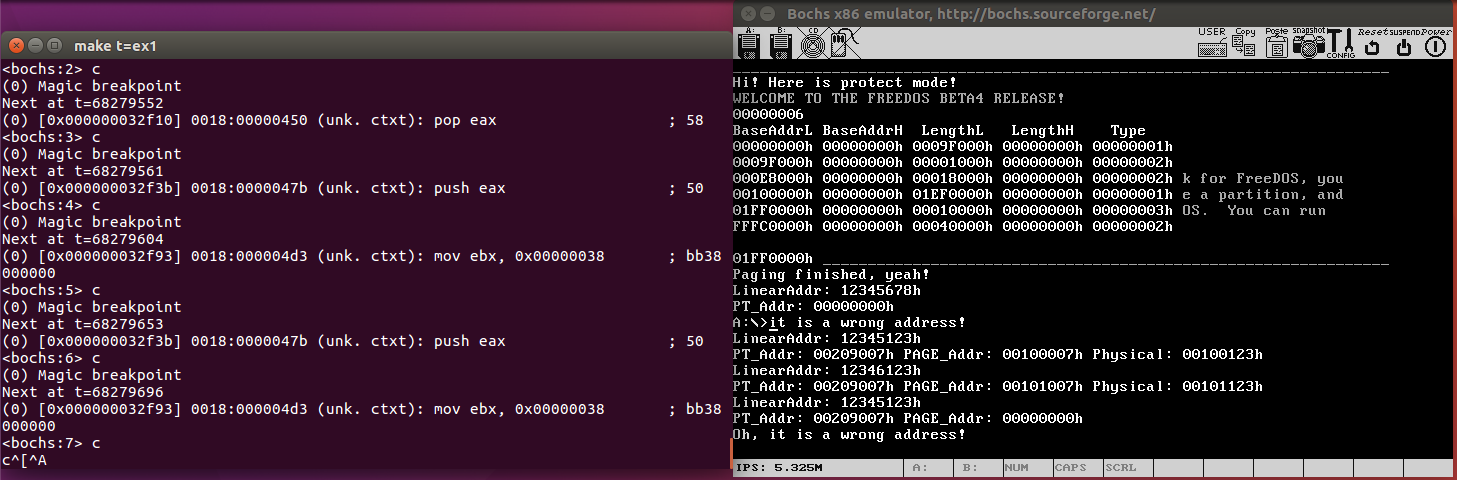
\includegraphics[width=12cm]{images/成功截图.png}
        \caption{成功运行的截图}
        \label{fig:my_label}
    \end{figure}
    
    除了内存显示的部分,截图下面的部分是下面代码的输出结果:
    \begin{lstlisting}[language={[x86masm]Assembler}]
    mov eax, 012345678h
    call TestL2P
    mov eax, 012345000h
    mov ecx, 2000h
    call alloc_pages
    test ebx, ebx
    jz .d1
    ShowStr strDEBUG
.d1:
    mov eax, 012345123h
    call TestL2P
    mov eax, 012346123h
    call TestL2P
    mov eax, 012345000h
    mov ecx, 2000h
    call free_pages
    mov eax, 012345123h
    call TestL2P
    \end{lstlisting}
    
    第一次查询 0x12345678时,由于页表和页目录都不存在,这个虚拟地址并没有对应值,程序提示找不到地址。第二、三次查询前,我们为 0x12345000 ~ 0x12346000的虚拟地址分配了物理内存,因此再次查询时,顺利计算出了物理地址。第三次查询前,我们释放了这里的物理内存,因此又无法找到物理内存了。
    
    \subsection{设计一个内存管理器}
    \subsubsection{原理阐述}
    
    Buddy 算法是一种广泛使用的内存管理算法,其特点是实现简单、效率高,但容易产生碎片。在伙伴系统中,可分配的内存空间是2的幂的大小的单个块。当接受到第一个请求时,如果请求的大小大于初始请求的一半,则分配整个块。否则,将该块拆分成两个绑定且相邻的“伙伴”块,如果请求的大小超过其中一个“伙伴”块的大小的一半,则将这个“伙伴”块直接分配给它,否则,其中一个“伙伴”块再次被分成两半。重复这个步骤,一直到找到满足请求大小的最小块,并分配出去。
    
    当回收内存块时,找到这块内存的“伙伴”块,如果“伙伴”块没有被分配出去,则这一对内存块可以进行合并。合并之后,可以继续判断合并后的内存块的“伙伴”块是否可以被合并。重复这个步骤,直到不能继续合并为止。

    \begin{figure}[H]
        \centering
        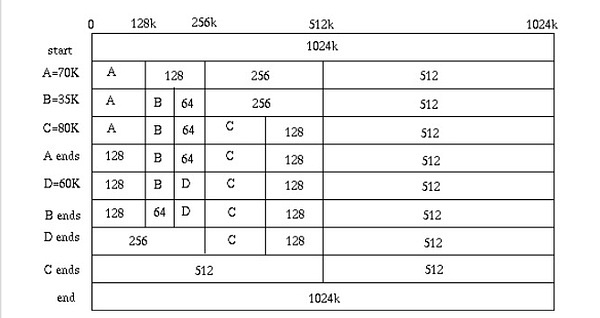
\includegraphics[width=12cm]{images/buddy.jpg}
        \caption{Buddy算法原理}
        \label{fig:buddy}
    \end{figure}
    
    图\ref{fig:buddy}描述了伙伴算法分配和回收的过程。
    
    \subsubsection{设计概述\label{设计概述}} 
    在\ref{Basic page switch}的基础上,我们选择采用伙伴(Buddy)算法进行物理内存的管理,实现了一个物理内存分配器。分配器采用了C语言实现,现阶段还无法整合到系统中,仅测试了接口的正确性。
    
    我们使用一系列位图来管理物理内存空间,如图\ref{fig:free_area}所示。位图中的一个二进制位对应了一块内存的使用情况,0表示这块内存未被分配。共有10个位图,每个位图所标明的内存粒度不同:位图的下标$i$表示大小为$2^i$字节的页框的使用情况,我们将这个下表值叫做$order$。例如,假设页面大小为4KiB,并且free\_area[2].maps的第0x30位为0,则表示物理内存上0xc0000$\sim$0xc3fff的位置是可用的。初始状态下,除了最大粒度的位图($order=9$)中的可用部分为0,不可用部分(为外设、BIOS等保留的地址)和其余位图均为1。
    
    \begin{figure}[H]
        \centering
        \begin{minipage}[t]{0.5\textwidth}
        \centering
        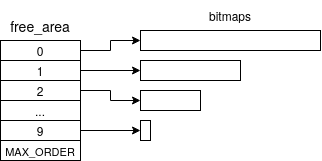
\includegraphics[height=3.5cm]{images/free_area.png}
        \caption{free\_area数组结构}
        \label{fig:free_area}
        \end{minipage}
        \begin{minipage}[t]{0.49\textwidth}
        \centering
        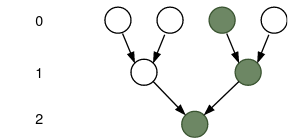
\includegraphics[height=3.5cm]{images/binary_tree.png}
        \caption{二叉树角度看bitmaps}
        \label{fig:binary_tree}
        \end{minipage}
    \end{figure}
    
    所有的bitmaps还可以以二叉树的视角来看待,如图\ref{fig:binary_tree}所示,其中实心表示位图对应二进制位值为1,空心表示值为0。每次分配时,先在请求的$order$层进行寻找,如果找到为0的二进制位,则直接将其设为1,表示这部分物理内存已经被分配出去,并返回地址;如果没有找到,则需要将更大块的内存分解,并将其中一块用于满足请求,而将另一块在位图对应位置上设为0,表示可以被分配。
    
    \subsubsection{代码实现}
    完整代码参见\href{https://www.github.com/xinyangli/orange-os}{GitHub}。
    
    基本数据结构和宏的声明如下:
    
    \begin{lstlisting}[language=C]
typedef struct {
  unsigned int *map;
  int size; /* size of bitmap array */
} free_area_t;
free_area_t free_area[MAX_ORDER]; /* array of free space bitmap */
    \end{lstlisting}
其中,map所指向的空间需要额外进行分配。

    如\ref{设计概述}中所述,外层的while循环从小块内存向大块内存搜索可用空间,corder表示现在正在搜索的order大小。一旦搜索到可用空间,则一层层回到$order$处,用设置位图上值的方式将过程中的大内存块分解。分配页面时,使用clz()函数计算位图数组高位中前导0个数,并存储在pos中。通过位运算pos $<<$ order $<<$ LPAGE\_SIZE即可得到位图某位对应的物理内存地址基址。
    
    \begin{lstlisting}[language=C]
PM alloc_pages(unsigned int order) {
  unsigned long pos = 0; /* position of available bit in bitmap*/
  unsigned int corder = order; /* current order to search */
  PM paddr = NULL;
  while(true) {
    pos = 0;
    for(int i = 0; i < free_area[corder].size; i++) {
      if (free_area[corder].map[i] == 0) {
        pos += 32;
      } else {
        pos += clz(free_area[corder].map[i]);
      }
    }

    if (pos == free_area[corder].size * 32) {
      /* no available space in request order */
      /* find in higher order and split */
      ++corder;
      continue;
    }

    SET_BIT(free_area[corder].map, pos);
    for(--corder; corder > order; --corder) {
      pos <<= 1;
      CLEAR_BIT(free_area[corder].map, pos ^ 1); /* set buddy to free */
    }
    return (PM)(pos << LPAGE_SIZE << order);
  }
}
    \end{lstlisting}

    在回收时,需要查看当前回收的内存的“伙伴”是否为空闲状态,如果是,则将这两个内存块合并,并继续到上一层查看是否可以合并。通过 pos\^1,即可得到“伙伴”块的位图位置。

    \begin{lstlisting}[language=C]
void free_pages(PM paddr, unsigned int order) {
  unsigned int corder = order;
  unsigned long pos = (unsigned long) paddr >> LPAGE_SIZE >> order;
  while(corder < MAX_ORDER) {
    if (TEST_BIT(free_area[corder].map, pos ^ 1)) {
      CLEAR_BIT(free_area[corder].map, pos);
      /* buddy is occupied, stop */
      break;
    }
    /* buddy is free */
    SET_BIT(free_area[corder].map, pos);
    ++corder; pos >>= 1;
  }
}
    \end{lstlisting}
    
    \section{实验结果总结}
    \subsection{分页机制}
    分页存储的逻辑是:将用户程序(进程)的 逻辑地址空间分成若干个大小相等的页(4KiB)并编号,同时将内存的物理地址也分成若干个块或页框(4KiB)并编号。再通过页表实现两者的一一映射关系,从而实现将进程的各个页离散地存储在内存的任一物理块中,有效提高了内存的利用率。
    \begin{figure}[H]
        \centering
        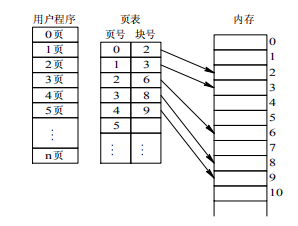
\includegraphics[width=8cm]{images/页表.png}
        \caption{页表}
        \label{页表}
    \end{figure}
    
    分页机制建立在分段机制的基础上。分页的开启与关闭由CR0寄存器的最高位PG标识。在未打开分页机制时,线性地址等同于物理地址,即逻辑地址通过分段机制直接转换成物理地址;分页开启后,分段机制将逻辑地址转换为线性地址,线性地址通过分页机制转换为物理地址。地址转换关系如图\ref{地址关系}所示。
    \begin{figure}[H]
        \centering
        
\includegraphics[width=12cm]{images/地址关系.png}
        \caption{地址关系}
        \label{地址关系}
    \end{figure}
    
    在线性地址转化成物理地址的过程中,分页机制使用页目录表和页表两级转换。其中页目录表的物理地址需要通过CR3寄存器也就是PDBR(Page Table Base Register)来确定。它的高20位将是页目录表首地址的高20位。
    \begin{figure}[H]
        \centering
        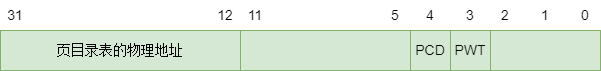
\includegraphics[width=12cm]{images/CR3.png}
        \caption{CR3的结构}
        \label{CR3结构}
    \end{figure}
    
    转换地址对应的示意图如图\ref{分页机制}所示。
    \begin{figure}[H]
        \centering
        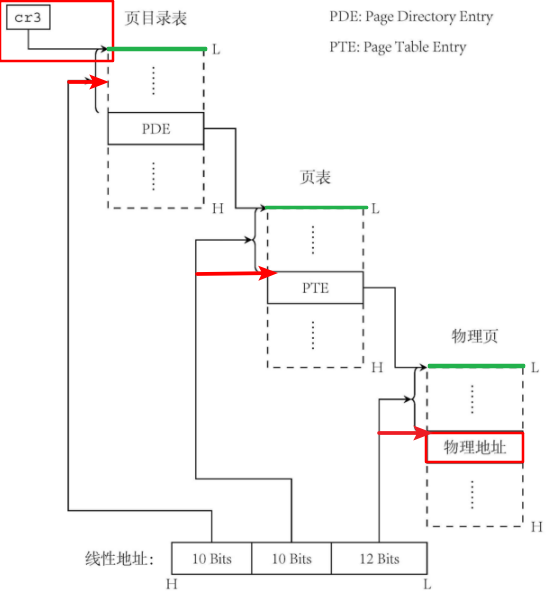
\includegraphics[width=12cm]{images/分页机制.png}
        \caption{分页机制}
        \label{分页机制}
    \end{figure}
    
    确定物理地址的步骤分为如下三步:
    
    $\bullet$ 从CR3中取出进程的页目录地址,根据线性地址前十位,在页目录表中找到对应的索引项;
    
    $\bullet$ 根据线性地址的中间十位,在页表(也是数组)中找到页的起始地址;
    
    $\bullet$ 将页的起始地址与线性地址中最后12位相加,得到最终的物理地址。
    
    PDE和PTE的结构如下:
    \begin{figure}[H]
        \centering
        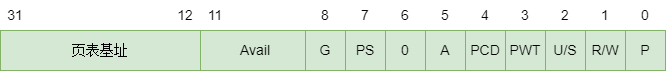
\includegraphics[width=14cm]{images/PDE.png}
        \caption{PDE结构}
        \label{PDE}
    \end{figure}
    \begin{figure}[H]
        \centering
        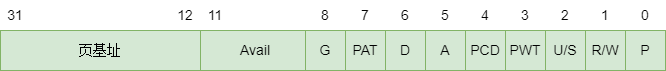
\includegraphics[width=14cm]{images/PTE.png}
        \caption{PTE结构}
        \label{PTE}
    \end{figure}
    
    关于不同位的含义,总结成下表:
    % Please add the following required packages to your document preamble:
% \usepackage[table,xcdraw]{xcolor}
% If you use beamer only pass "xcolor=table" option, i.e. \documentclass[xcolor=table]{beamer}
\begin{table}[H]
\caption{不同位的含义解释}
\centering
\begin{tabular}{|c|c|}
\hline
\multicolumn{1}{|c|}{{\color[HTML]{000000} \textbf{名称}}} & \multicolumn{1}{c|}{{\color[HTML]{000000} \textbf{含义}}}          \\ \hline
{\color[HTML]{000000} P}                                 & {\color[HTML]{000000} 存在位标志,表示当前条目所指向的页或页表是否在物理内存中}             \\ \hline
{\color[HTML]{000000} R/W}                               & {\color[HTML]{000000} 读写位标志,指定一个页或者一组页的读写权限。}                   \\ \hline
{\color[HTML]{000000} U/S}                               & {\color[HTML]{000000} 用户/超级用户标志,指定一个页或者一组页的特权级}                 \\ \hline
{\color[HTML]{000000} PWT}                               & {\color[HTML]{000000} 标志对单个页或者页表的Write-back或Write-through缓冲策略}  \\ \hline
{\color[HTML]{000000} PCD}                               & {\color[HTML]{000000} 用于控制对单个页或者页表的缓冲}                          \\ \hline
{\color[HTML]{000000} A}                                 & {\color[HTML]{000000} Access,标志页或者页表是否被访问}                      \\ \hline
{\color[HTML]{000000} D}                                 & {\color[HTML]{000000} Dirty,标志页或者页表是否被写入}                       \\ \hline
{\color[HTML]{000000} PAT}                               & {\color[HTML]{000000} Page Table Atttribute Index,实验中将该位设为0即可。} \\ \hline
{\color[HTML]{000000} PS}                                & {\color[HTML]{000000} Page Size,页大小。PS=0时页大小为4KiB,PDE指向页表。}      \\ \hline
{\color[HTML]{000000} G}                                 & {\color[HTML]{000000} 指示全局页。}                                   \\ \hline
{\color[HTML]{000000} AVL}                               & {\color[HTML]{000000} 保留字段。}                                    \\ \hline
\end{tabular}
\end{table}

至此,关于分页机制的基本知识已经较为全面地给出。

    \subsection{分页机制的基本方法和思路}
    pmtest6.asm中给出了基本的分页机制方法和思路。大致总结如下:初始化PDE $\rightarrow$ 初始化PTE $\rightarrow$ 正确设置CR3的值,指向页目录表基地址 $\rightarrow$ 修改CR0最高位为1,开启分页。
    
    \subsection{PDE和PTE的计算方法}
    pmtest6.asm内存映射图如图\ref{pmtest6_mem}所示。每个PDE前20位表示对应的页表的基地址。每个页表包含1024个PTE。每个PTE指向一个页。在pmtest6中,1024个页表占用4M的空间,它们一共可以指向1024*1024个页,对应4GB的空间。关于寻址的计算方法在\ref{分页机制}也已经提及。
    
    Q:为什么代码3.22里面,PDE初始化添加了一个PageTblBase(Line212),而PTE初始化时候没有类似的基地址呢(Line224)?
    
    A:PDE初始化添加了一个PageTblBase(Line 212)是因为页表起始地址为PageTblBase(0x201000h,即2M+4K)。而在PTE初始化时,由于pmtest6中物理地址等于线性地址,PTE的起始地址就是0。所以可以省略基地址。
    
    \subsection{获取内存布局的方法}
    参照pmtest7的方法,可以调用中断15h来获取内存信息。
    调用该中断需要设置如下参数:
    
    $\bullet$ eax:要想获取内存信息,需要将ax赋值为0E820h。
    
    $\bullet$ ebx:放置“后续值”,第一次调用需要设置ebx为0。
    
    $\bullet$ es:di:指向一个ARDS。
    
    $\bullet$ ecx:es:di所指向的地址范围描述符结构的大小,以字节为单位。
    
    $\bullet$ edx:0534D4150h('SMAP')——BIOS将会使用此标志,对调用者将要请求的系统映像信息进行校验,这些信息会被BIOS放置到es:di所指向的结构中。
    
    中断调用之后,结果存放于下列寄存器之中。
    
    $\bullet$ CF:CF=0表示没有错误,否则存在错误。
    
    $\bullet$ eax:0534D4150h('SMAP')。
    
    $\bullet$ ecx:BIOS 填充在地址范围描述符中的字节数量。
    
    $\bullet$ ebx:这里放置着为等到下一个地址描述符所需要的后续值。
    
    ARDS的结构为:
    \begin{table}[H]
    \centering
    \begin{tabular}{|c|c|c|}
    \hline
    {\color[HTML]{333333} \textbf{偏移}} & {\color[HTML]{333333} \textbf{名称}} & \textbf{意义} \\ \hline
    0   & BaseAddrLow     & 基地址的低32位    \\ \hline
    4   & BaseAddrHigh     & 基地址的高32位    \\ \hline
    8   & LengthLow     & 长度的低32位     \\ \hline
    12   & LengthHigh   & 长度的高32位     \\ \hline
    16         & Type   & 这个地址范围的地址类型 \\ \hline
    \end{tabular}
    \end{table}
    
    其中Type不同取值的含义见下表:
\begin{table}[H]
\centering
\begin{tabular}{|c|c|p{8cm}<{\centering}|}
\hline
{\color[HTML]{333333} \textbf{取值}} & {\color[HTML]{333333} \textbf{名称}} & \textbf{意义}                   \\ \hline
1    & AddressRangeMemory    & 这个内存段是可以被OS使用的RAM             \\ \hline
2   & AddressRangeReserved & 这个地址段正在被使用,或者被系统保留所以一定不能被OS使用 \\ \hline
其他                                 & 未定义                                & 保留,为未来使用                      \\ \hline
\end{tabular}
\end{table}
    因为int 15h需要将内存段描述保存到缓冲区中,所以在调用该中断前,需要准备好缓冲区。我们可以将所有ARDS保留在同一片缓冲区中,但是要保证缓冲区大小充足。
    


    \section{思考题汇总}
    \begin{enumerate}
        \item 分页和分段有何区别?在本次实验中,段页机制是怎么搭配工作的?
        
        $\bullet$ 区别:
        % Please add the following required packages to your document preamble:
% \usepackage[table,xcdraw]{xcolor}
% If you use beamer only pass "xcolor=table" option, i.e. \documentclass[xcolor=table]{beamer}
\begin{table}[H]
\centering
\begin{tabular}{|p{7cm}<{\centering}|p{7cm}<{\centering}|}
\hline
\textbf{分页} & \textbf{分段}            \\ \hline
在分页中,进程的地址空间被划分为固定大小的页面            & 在分段中,进程的地址空间被划分为大小不同的段 \\ \hline
操作系统负责分页                           & 编译器负责分段                \\ \hline
页大小由硬件决定                           & 段大小由用户给出               \\ \hline
速度比分段块                             & 分段速度慢                  \\ \hline
分页会导致内部碎片                          & 分段导致外部碎片               \\ \hline
分页中,逻辑地址被划分为页号和页偏移                 & 分段中,逻辑地址被划分为段号和段偏移     \\ \hline
分页包含一个页表,页表包含每个页的基地址               & 分段包含段表,段表中包含段号和段偏移量    \\ \hline
分页对于用户不可见                          & 分段对于用户可见               \\ \hline
在分页中,处理器需要页号和页偏移来计算实际物理地址          & 分段中,处理器使用段号和段偏移量计算地址   \\ \hline
\end{tabular}
\end{table}
    段页式如何搭配:分段和分页相结合,其地址结构由:段号、段内页号、页内地址三部分组成。在段页式系统中获得一条指令需要三次访问内存,第一次访问内存中的段表,第二次访问内存中的页表,第三次访问内存中的数据。
        
    \item PDE、PTE,是什么?例程中如何进行初始化?CPU是怎样访问到PDE、PTE,从而计算出物理地址的?
    
    $\bullet$ PDE是页目录表中的表项,PTE是页表中的表项。初始化需要loop循环依次赋值,具体可以参考\ref{调试PTE,PDE}节的细节阐述。
    
    \item 开启分页机制之后,在GDT表中、在PDE、PTE中存的地址是物理地址、线性地址,还是逻辑地址,为什么?

    GDT表中是线性地址,PDE和PTE中的地址是物理地址。GPT是段式管理用到的,而分段就是将逻辑地址转换为线性地址。PDE是定位PTE的,存放的是PTE的物理地址,PTE是定位页的,存放的是页的物理地址。
    
    \item 为什么PageTblBase初始值为2M+4K?能不能比这个值小?
    
    不能。因为设置页目录表起始地址是2M,且页目录表大小为4K。所以PageTblBase初始值必须大于等于2M+4K。否则PTE与PDE存放位置会有交叉,导致错误。
    
    \item 怎么读取本机的实际物理内存信息?
    
    在\ref{运行pmtest7}节中,我们使用的是int 15h,ax=0xE820h的中断。它可以得到ARDS的列表,这也是当下主流的查看内存的方法。事实上,在早期计算机上,还有许多其他函数(“int 0x12”,“int 0x15,ax=0xE881”,“int 0x15,ax=0xE801”,“int 0x15,ah=0xC7”,“int 0x15,ah=0x8A ", "int 0x15, ax=0xDA88", "int 0x15, ah=0x88")可以实现这一功能。不过,所有这些都在1990 年代初被弃用了。
    
    \item 如何进行地址映射与切换?
    
    参考\ref{运行pmtest8}节内容,地址映射与切换的原理在其中已经清楚地阐述过了。
    
    \end{enumerate}
    
    
    \section{实验问题总结}
    \begin{enumerate}
    \item 如果线性地址$=$物理地址不成立,那么在切换页表时需要哪些额外的操作?
    
    经过我们的初步讨论,有以下可行方案:可以关闭分页,直接操作物理内存地址;把PTE和PDE的地址设置为与线性地址一一对应;把PTD和PDE的地址存在特定虚拟地址上。
    
    \item 在打开分页模式后,示例代码中使用了如下的短跳转。这个短跳转的意义是什么?如果不加是否能正确运行?
    \begin{lstlisting}[language={[x86masm]Assembler}]
    jmp	short .3
.3:
	nop
    \end{lstlisting}
    针对这个问题,我们提出了以下猜想
    $\bullet$ 出于内存对齐的原因。不过在讨论后,我们觉得内存对齐应该由汇编器负责,而不应该手动添加。
    $\bullet$ 通过短跳转刷新指令寄存器。短跳转也许可以将指令寄存器中的值从物理地址切换到虚拟地址。不过,我们在试验之后,发现去掉jmp后仍能运行。针对这个现象,有组员提出,能够运行或许是由于线性地址$=$物理地址,有待进一步验证。
    $\bullet$ 有可能是希望借助jmp刷新CPU指令缓存。因为在启用分页前后,缓存会从Physically tagged转换为Virtually tagged。jmp可能会刷新缓存,加速运行。有待进一步验证。    
    \item 代码中初始化页表时使用了mul ebx,其中ebx中的值为1024。这个命令可以改成shl eax,10吗?
    
    我们感觉可以。
    \end{enumerate}

    
    \section{各人实验贡献与体会}
    通过本次实验,对操作系统的段页式管理的原理和代码实现有更深刻的理解。在获取系统内存布局后,能够对PDE、PTE的数量有更加合理的设置,从而减小程序占用内存空间。通过对pmtest8的调试,对地址映射关系以及内存管理更加熟悉。在进阶题的思考过程中,我们对内存分配的几种方式又进行了回顾。
    
    本次实验中,李心杨负责编写内存管理器;王宇骥调试pmtest6、pmtest7相关内容,回答相关思考题;郑炳捷调试pmtest8相关内容,回答相关思考题;林锟杨负责基础题的编程任务,完整实现了整个程序。
    
    %% 结束表格
    \begin{table}[H]
    \centering
    \begin{tabular}{|p{4cm}<{\centering}|p{6cm}<{\centering}|p{3cm}<{\centering}|}
    \hline
    \multicolumn{3}{|c|}{\textbf{教师评语}}                                                  \\ \hline
    \multicolumn{3}{|c|}{ \rule{0pt}{60pt} }  \\ \hline
    {\textbf{姓名}} & {\textbf{学号}}   & \textbf{分数} \\ \hline
    \multicolumn{1}{|c|}{李心杨} & \multicolumn{1}{c|}{2020302181022}  &             \\ \hline
    \multicolumn{1}{|c|}{王宇骥} & \multicolumn{1}{c|}{2020302181008} &             \\ \hline
    \multicolumn{1}{|c|}{林锟扬} & \multicolumn{1}{c|}{2020302181032} &             \\ \hline
    \multicolumn{1}{|c|}{郑炳捷} & \multicolumn{1}{c|}{2020302181024} &             \\ \hline
    \multicolumn{3}{|l|}{教师签名:}       \\ 
    \multicolumn{3}{|r|}{} \\ 
    \multicolumn{3}{|r|}{年 \space 月 \space 日} \\ \hline
    \end{tabular}
    \end{table}
\end{document}